\documentclass{article}
\usepackage{mathrsfs}
\usepackage{harpoon}
%\usepackage{ctex}
\usepackage{color}
\usepackage{amsmath}
\usepackage{mathtools}
\usepackage{simplewick} 
\usepackage{graphicx} % added for subfig
\usepackage{subfigure} % added for subfig
\title{Note for g.s. fit}
\author{Tony Chu and Jinchen He\\ \small Tusng-Dao Lee Institude \& Shanghai Jiao Tong University}
\date{\today}
\usepackage[a4paper,left=20mm,right=20mm,top=20mm,bottom=20mm]{geometry}
\begin{document}
\maketitle
\tableofcontents
\pagebreak[4]
\section{Choice of fit method}

\subsection{Fit function}
In the two states fit method, we did joint fit with three parts: local matrix element $C(z=0, t)$, real and imag part of ratio $\frac{C(z, t)}{C(z=0, t)}$. 
\begin{enumerate}
    \item For local part
    \[ C(z=0, t) = c e^{-E_{0} t}\left(1+a_{1} e^{-\Delta E t}\right) \]
    \item For real/imag part of ratio
    \[ \frac{C(z, t)}{C(z=0, t)} = \frac{\phi_{2}\left(1+b_{1 (re/im)} e^{-\Delta E t}\right)}{1+a_{1} e^{-\Delta E t}} \]
\end{enumerate}

In the one state fit method, we fit real/imag part of ratio directly,
\[ \frac{C(z, t)}{C(z=0, t)} = \phi_{2 (re/im)} \]

One state fit v.s. two states fit, which shoule we choose in the analysis of two point data? Two figures are helpful before we set about doing fits:

\begin{enumerate}
    \item Effective mass plot of local matrix element.
    \[ \ln(\frac{C(z=0, t)}{C(z=0, t+1)}) = E_0 + \ln(1 + a_1 e^{-\Delta E t}) - \ln(1 + a_1 e^{-\Delta E t - \Delta E}) \]
    Therefore, if the effective mass plot is horizontal without decay behavior through t-axis, it is impossible to extract excited state contamination successfully.
    \item Effective mass plot of non-local matrix element.
    
\end{enumerate}



%%%%%%%%%%%%%%%%%%%%%%%%%%%%%%%%%%%%
%%%%%%%%%%%%%%%%%%%%%%%%%%%%%%%%%%%%
\subsection{Example 1}

\begin{figure}[htbp]
    \centering
    \subfigure[Local matrix element]{
    \begin{minipage}[t]{0.5\linewidth}
    \centering
    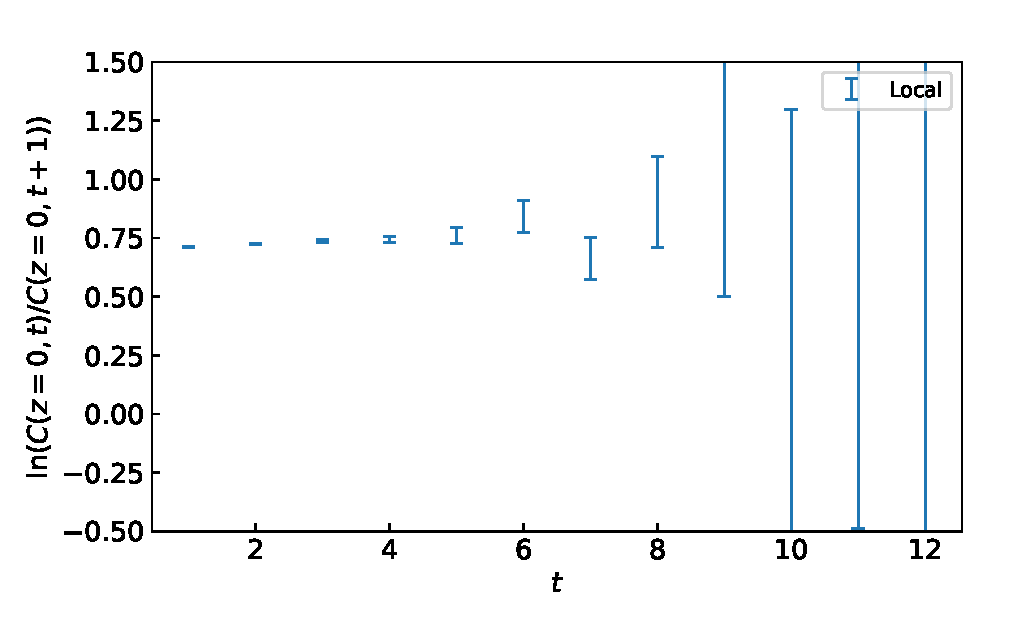
\includegraphics[width=3.2in]{fit_fig/b_local_meff.pdf}
    %\caption{fig1}
    \end{minipage}%
    }%
    \subfigure[Non-local matrix element]{
    \begin{minipage}[t]{0.5\linewidth}
    \centering
    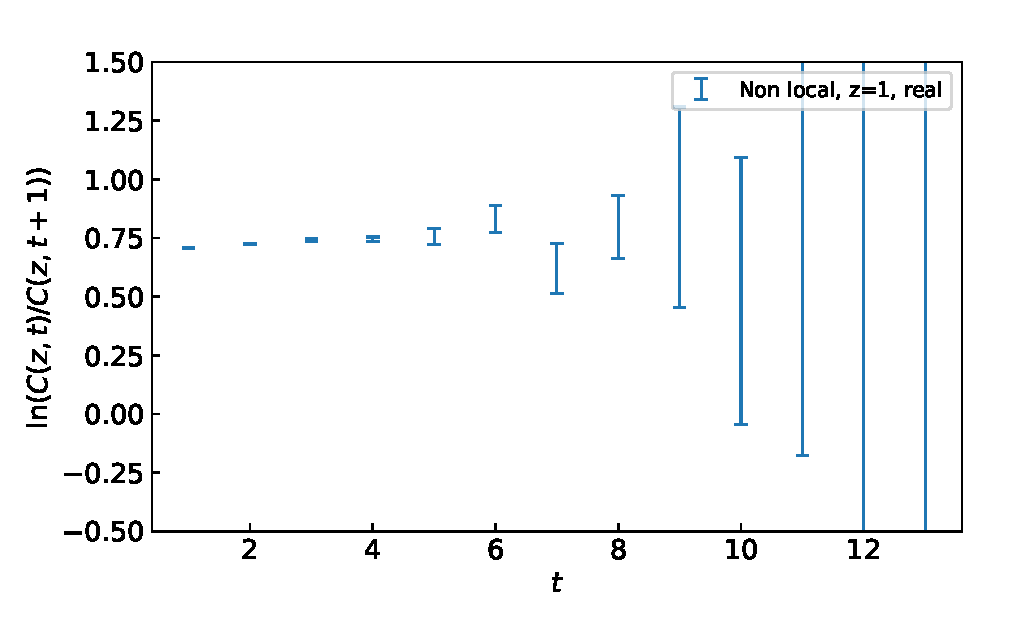
\includegraphics[width=3.2in]{fit_fig/b_non_local_meff.pdf}
    %\caption{fig2}
    \end{minipage}%
    }%
    \centering
    \caption{Effective mass}
\end{figure}

Neither of two plots of effective mass above shows the exponential decay behavior at small t region, so the one state fit method is suggested.

\begin{figure}
    \centering
    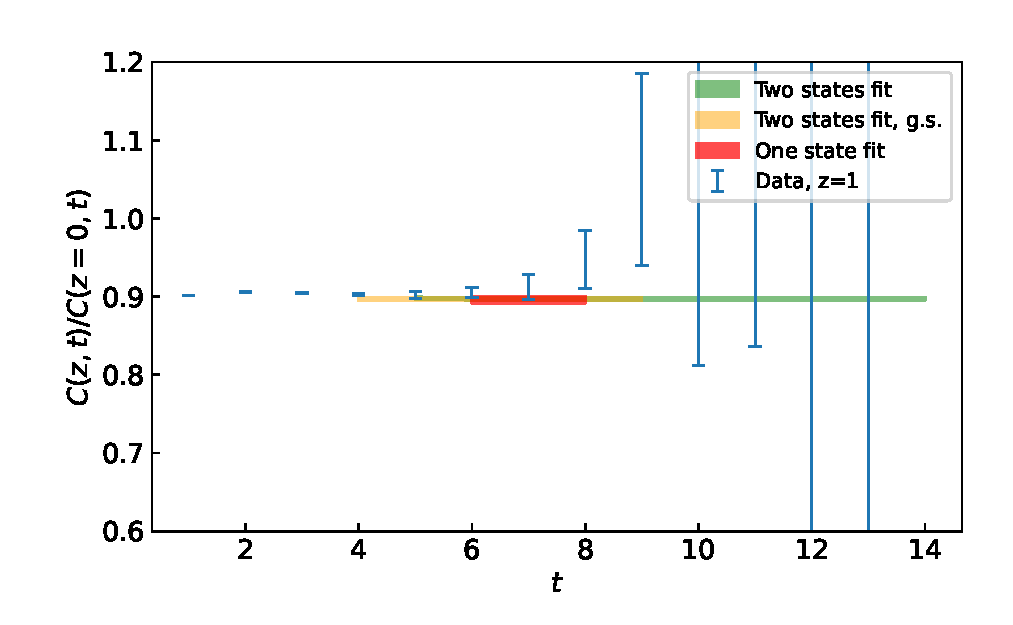
\includegraphics[height=7cm,width=11.3cm]{fit_fig/b_fit_result.pdf}
    \caption{Fit result comparison}
\end{figure}

This is the output of two states fit,
\begin{equation}
    \begin{aligned}
    &\text { Least Square Fit: } \\
    &\text { chi2/dof [dof] }=0.91[18] \quad Q=0.57 \quad \log G B F=96.901 \\
    &\text { Parameters: } \\
    &\text { $g.s._{re}$ } \quad 0.8964 (25) \\
    &\text { $a1$ } \quad -2.6 (6.5) \\
    &\text { $b1_{re}$ } \quad -1.6 (4.1) \\
    &\text { $dE1$ } \quad 1.30 (73) \\
    &\text { $E0$ } \quad 0.7442 (82)
    \end{aligned}
\end{equation}

From the output it can be found that the fit result of excited state's coefficient $b_1$ covers zero within the error, which means the two states fit failed to extract the excited state contamination.






%%%%%%%%%%%%%%%%%%%%%%%%%%%%%%%%%%%%
%%%%%%%%%%%%%%%%%%%%%%%%%%%%%%%%%%%%
\subsection{Example 2}

\begin{figure}[htbp]
    \centering
    \subfigure[Local matrix element]{
    \begin{minipage}[t]{0.5\linewidth}
    \centering
    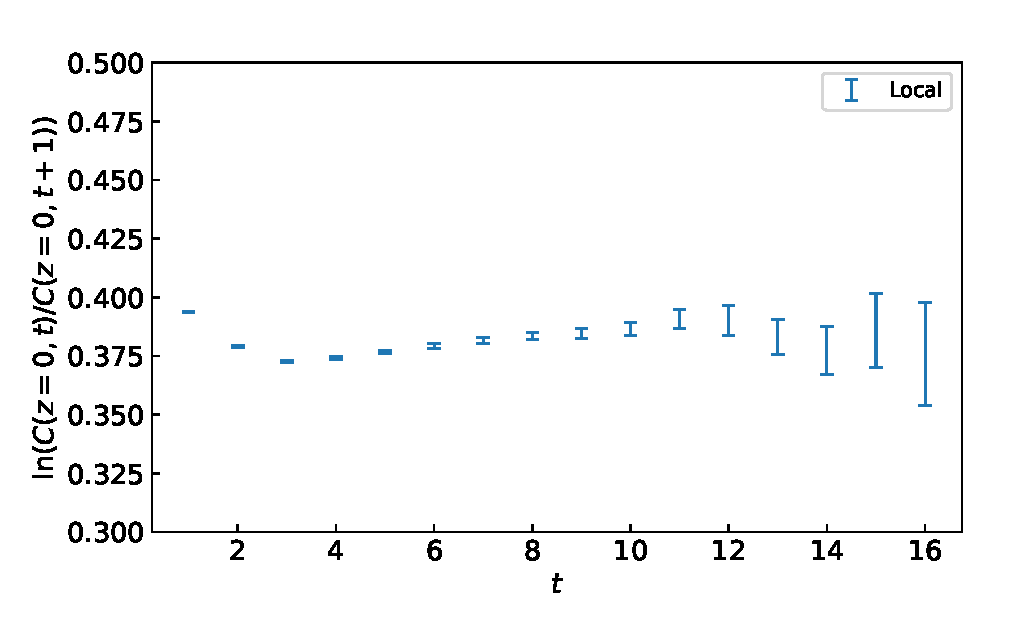
\includegraphics[width=3.2in]{fit_fig/g_local_meff.pdf}
    %\caption{fig1}
    \end{minipage}%
    }%
    \subfigure[Non-local matrix element]{
    \begin{minipage}[t]{0.5\linewidth}
    \centering
    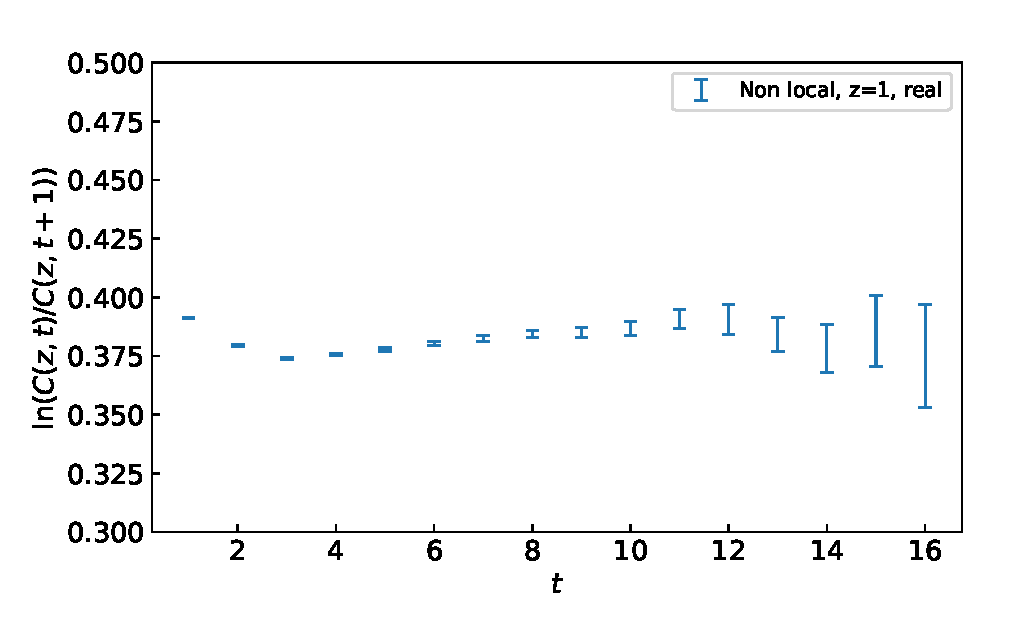
\includegraphics[width=3.2in]{fit_fig/g_non_local_meff.pdf}
    %\caption{fig2}
    \end{minipage}%
    }%
    \centering
    \caption{Effective mass}
\end{figure}

Both of two plots of effective mass above shows the exponential decay behavior at small t region, so the two states fit is worthy to try.

\begin{figure}
    \centering
    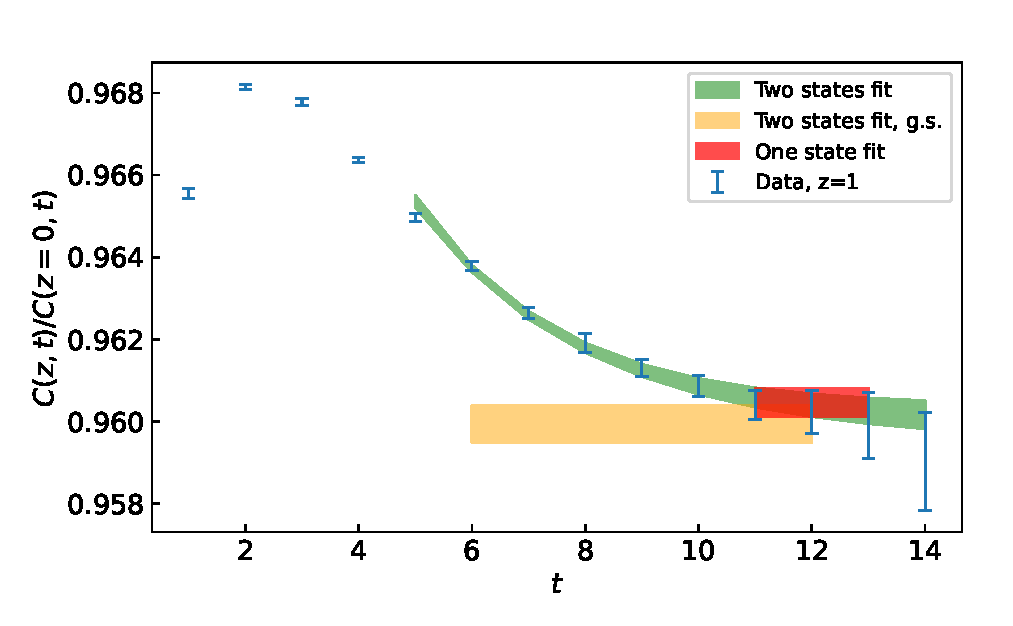
\includegraphics[height=7cm,width=11.3cm]{fit_fig/g_fit_result.pdf}
    \caption{Fit result comparison}
\end{figure}

This is the output of two states fit,
\begin{equation}
    \begin{aligned}
    &\text { Least Square Fit: } \\
    &\text { chi2/dof [dof] }=0.2[21] \quad Q=1 \quad \log G B F=194.25 \\
    &\text { Parameters: } \\
    &\text { $g.s._{re}$ } \quad 0.95954 (56) \\
    &\text { $a1$ } \quad -0.231 (41) \\
    &\text { $b1_{re}$ } \quad -0.206 (40) \\
    &\text { $dE1$ } \quad 0.294 (53) \\
    &\text { $E0$ } \quad 0.3899 (20)
    \end{aligned}
\end{equation}

From the output it can be found that the fit result of excited state's energy $\Delta E$ and coefficient $b_1$ does not cover zero within the error, which means the two states fit succeeded to extract the excited state contamination.

\end{document}